\chapter{系统操作}
\section{系统起动}
\begin{itemize}
    \item 在桌面找到\lstinline{multimeter.exe}的快捷方式
    \item 在安装路径根目录找到\lstinline{multimeter.exe}应用程序
\end{itemize}
以上两种方式均可打开本软件。
\section{基本操作}
\subsection{用户登录}
打开本软件后,首先要选择用户模式并登录。本软件有以下两种用户模式:
\begin{itemize}
    \item 普通用户
    \item 高级用户
\end{itemize}
使用者可通过下拉选项选择。
\begin{figure}[htbp]
    \centering
    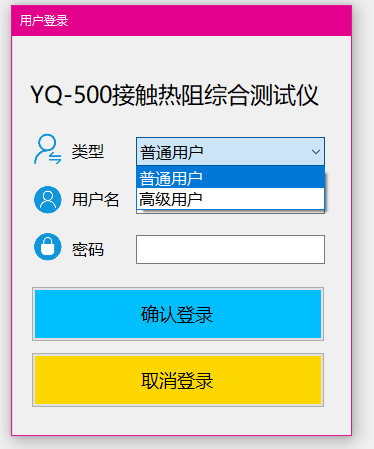
\includegraphics[width=0.8\textwidth]{operation/login.png}
    \caption{ 用户登录 \label{fig:login}}
\end{figure}
相对\lstinline{普通用户},\lstinline{高级用户}可以进行更多系统级的设置,详见\ref{subsec:advancedUser}一节。

在对应栏输入账号密码后,按\lstinline{确认登录}按钮即可进入测试方法选择(见\ref{subsec:testMethods}),
按\lstinline{取消登录}按钮会直接退出本软件。
\begin{note}
    当前版本不支持用户的注册。在当前版本中\lstinline{普通用户}无需账号密码即可登录,\lstinline{高级用户}的账号密码均为\lstinline{admin}。
\end{note}
\subsection{测试方法\label{subsec:testMethods}}
本综合测试平台共支持四种测试方法:
\begin{itemize}
    \item 试件热导率测试
    \item 固-固试件间接触热阻测试
    \item 热流计间热界面材料测试
    \item 固-固试件间热界面材料测试
\end{itemize}
\begin{figure}[htbp]
    \centering
    \includegraphics[width=1\textwidth]{operation/chooseMethod.png}
    \caption{ 测试方法选择 \label{fig:chooseMethod}}
\end{figure}
其原理由\figref{fig:kappa}--\figref{fig:ITMS}所示:
\begin{figure}[H]
    \centering
    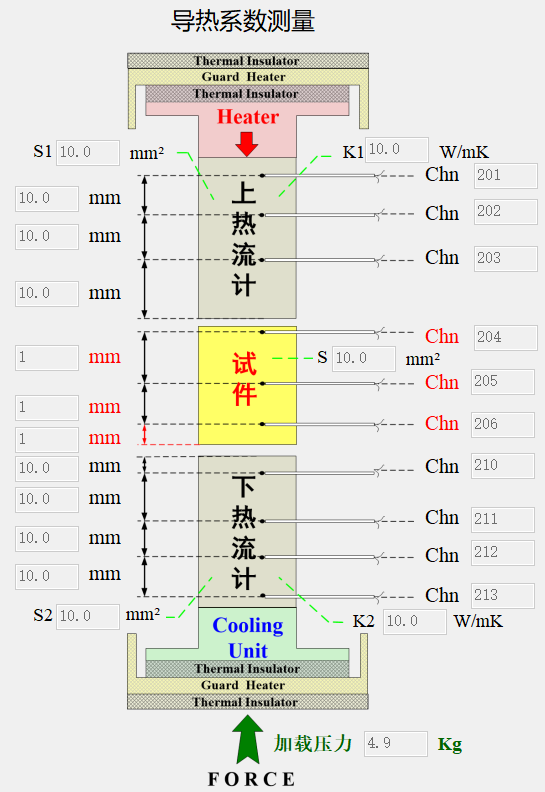
\includegraphics[width=1\textwidth]{operation/kappa.png}
    \caption{ 试件热导率测试原理图 \label{fig:kappa}}
\end{figure}
\begin{figure}[H]
    \centering
    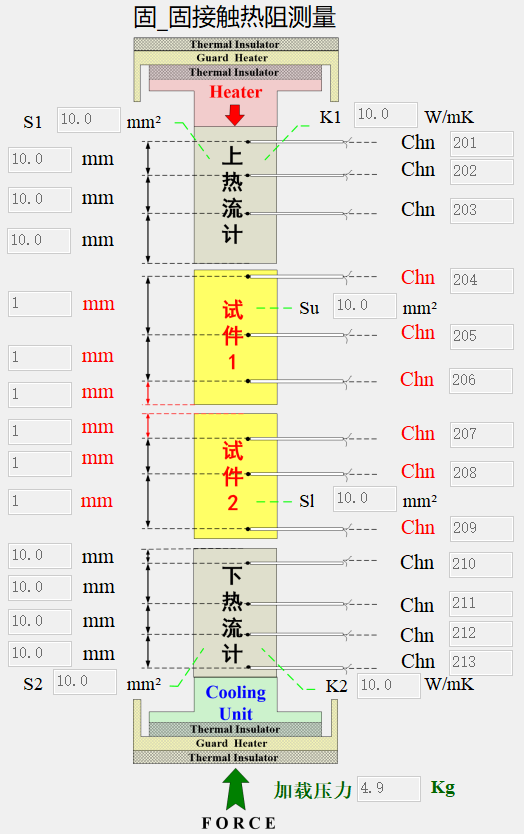
\includegraphics[width=1\textwidth]{operation/ITC.png}
    \caption{ 固-固试件间接触热阻测试原理图 \label{fig:ITC}}
\end{figure}
\begin{figure}[H]
    \centering
    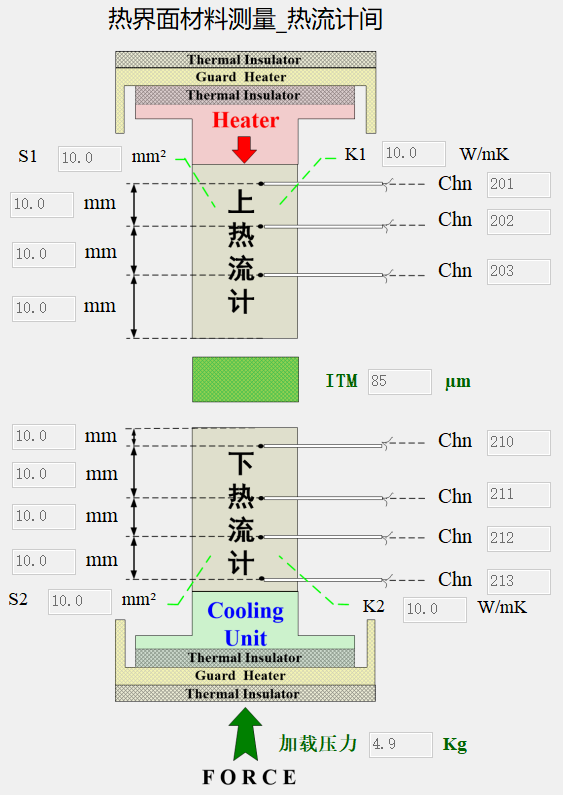
\includegraphics[width=1\textwidth]{operation/ITM.png}
    \caption{ 热流计间热界面材料测试原理图 \label{fig:ITM}}
\end{figure}
\begin{figure}[H]
    \centering
    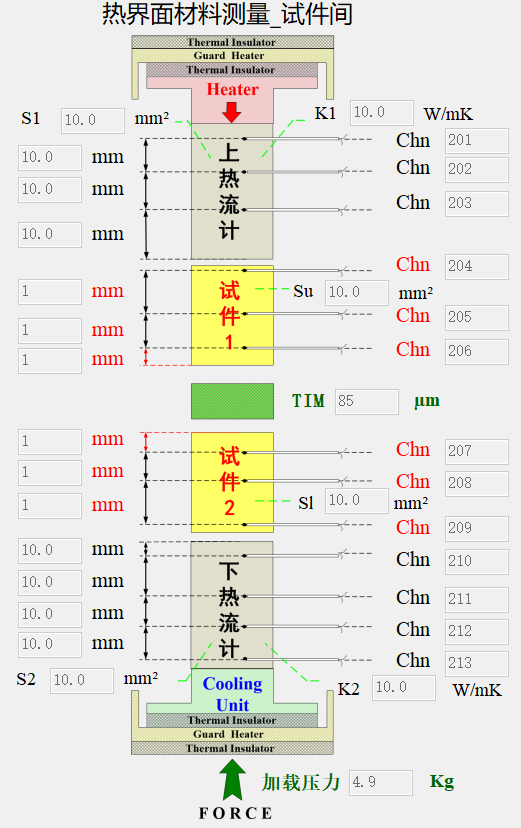
\includegraphics[width=1\textwidth]{operation/ITMS.png}
    \caption{ 固-固试件间热界面材料测试原理图 \label{fig:ITMS}}
\end{figure}
选择对应的测试方法可进入对应的页面,进行测试参数的设置,测试的启动/停止及测试结果的处理。
\subsection{切换测试方法}
在进入某一测试方法的页面后,若要改变测试方法,可点击\lstinline{切换方法}按钮(如\figref{fig:btnSwitchMethod}所示)
返回至方法选择界面(\figref{fig:chooseMethod})。
\begin{figure}[htbp]
    \centering
    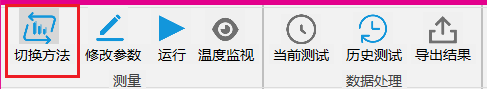
\includegraphics[width=1\textwidth]{operation/switchMethod.png}
    \caption{ 切换方法按钮 \label{fig:btnSwitchMethod}}
\end{figure}

\subsection{修改参数}
在选定测试方法后,可通过\lstinline{修改参数}按钮(如\figref{fig:btnChangePara}所示)修改实验的相关参数。
可供修改的参数在不同用户模式下也不相同。
\lstinline{普通用户}模式不支持热流计属性的修改,而\lstinline{高级用户}模式支持热流计属性的修改。
\begin{figure}[htbp]
    \centering
    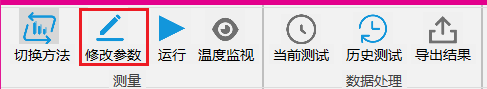
\includegraphics[width=1\textwidth]{operation/changePara.png}
    \caption{ 修改参数按钮 \label{fig:btnChangePara}}
\end{figure}
按下该按钮后,可供更改的参数将变为可编辑状态。可供编辑的参数如表\ref{tab:editableParaNormalUser}所示:
\begin{table}
    \centering
    \caption{ 可供修改的参数及其含义 \label{tab:editableParaNormalUser}}
    \begin{tabular}{@{}lc@{}}
        \toprule
        参数  & 含义                                                     \\ \midrule
        Su    & 上试件截面积                                             \\
        Sl    & 下试件截面积                                             \\
        S     & 试件面积                                                 \\
        ITM   & 热界面材料厚度                                           \\
        Force & 加载压力                                                 \\
        chn   & 热敏电阻测试通道(标签A$\sim$M分别对应通道201$\sim$213) \\
        mm    & 示意图中对应距离的数值                                   \\ \bottomrule
    \end{tabular}
\end{table}[htbp]
同时,\lstinline{修改参数}按钮变为\lstinline{确定参数}按钮。
当修改对应参数后,按\lstinline{确定参数}按钮,若无错误消息提示,则参数保存成功。
设置会保存在系统内,下一次实验会使用相同的参数。若无需改变参数,则可跳过该按钮,直接开始测试。

\begin{figure}[htbp]
    \centering
    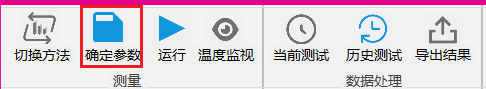
\includegraphics[width=1\textwidth]{operation/ensurePara.png}
    \caption{ 确定参数按钮 \label{fig:ensurePara}}
\end{figure}

\begin{note}
    若输入的参数有误,系统会弹出错误提示弹窗,如\figref{fig:errorParaSet}所示。此时请仔细检查设置的数据,
    修改正确后再保存。参数可能的错误原因及相应弹窗消息列在表\ref{tab:errorInfoNormalUser}中。
\end{note}

\begin{figure}[htbp]
    \centering
    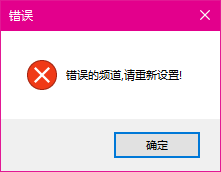
\includegraphics[width=1\textwidth]{operation/errorParaSet.png}
    \caption{ 参数设置错误时的弹窗 \label{fig:errorParaSet}}
\end{figure}
\begin{table}[htbp]
    \centering
    \caption{ 错误弹窗消息及可能的参数错误 \label{tab:errorInfoNormalUser}}
    \begin{tabular}{@{}lcc@{}}
        弹窗消息               & 错误参数   & 错误原因                     \\
        错误的数值,请重新设置! & Su,Sl,S,mm & 输入的不是一个数字           \\
                               & ITM,Force  & 输入的数字小于或等于0        \\
        错误的频道,请重新设置! & chn        & 输入的不是一个正整数         \\
                               &            & 通道编号不在201$\sim$213之间 \\
                               &            & 有重复的频道
    \end{tabular}
\end{table}
\begin{note}
    本软件支持任意的频道顺序,但为获得更好的使用体验,
    建议测试通道自上到下按201~213(对应热敏电阻A~M)由小到大排列。
\end{note}
\subsection{运行}
当测试参数保存成功后,按下\lstinline{运行}按钮后可开始进行检测。若没有修改参数,测试按当前显示的参数进行。
此后,运行按钮变为结束按钮,同时页面变为实时温度的图表
\subsection{温度监控}
\subsection{当前测试}
\subsection{历史测试}
\subsection{导出结果}
\subsection{高级用户模式\label{subsec:advancedUser}}
\subsubsection*{测试修改参数}
\subsubsection*{串口设置修改}
\subsubsection*{标定参数修改}
\section{各种数据}在软件的使用过程中,用户必须与各种数据和信息打交道。为了让用户能
够操作我们的软件,我们必须为用户提供各种结构以及每个数据元素的含义。
有些数据适合在系统操作说明中给出,有些适合在后面的附录中给出,甚至有些除了在
操作说明的同时给出外,还要在附录中给予归纳,这些都由用户手册编写人员根据实际
兄来决定。这些数据包括
输出数据:应当给出软件以何种形式输出的数据的内容和格式,并要求以例样的形式
给予说明。
中间数据〖条件〗:如果我们告诉用户在软件的运行过程中所产生的中间数据的内容
和格式,有助于用户理解软件的使用,则应当给予说明。
数据限制〖条件〗:如果对数据有限制,如数据的大小限制,则应当给予说明。
数据文件〖条件〗:如果要告诉用户我们的软件所使用的某些数据文件的结构有助于
用户理解我们软件的使用,则应给予说明,但应该注意技术保密。如果对数据文件有
所限制,例如每个文件的最大记录数、每个磁盘的最大文件数等,应当给予说明
\section{处理过程}
如果我们简要地给用户描述我们软件对用户的操作、输入的命令
和输入数据的处理过程,有助于用户了解我们软件的使用,则应给予说明
\section{出错处理}
应当给出各种出错情况以及相应的处理措施
\section{操作技术}
有些软件的操作可能需要一定的技术和经验,才能获得满意的结
果,那么应该在用户手册上尽量给出这些技术和经验的描述,或告诉用户如何才能获得
这些技术和经验。例如,在操作SEAS系统作图纸净化处理时,如何选择适当的阀值就是
需要一定的技术和经验的问题。